\documentclass[10pt]{article}
\usepackage[a4paper,margin=20mm]{geometry}
\usepackage[T1]{fontenc}
\usepackage[utf8]{inputenc}
\usepackage{lmodern,microtype,booktabs,graphicx,hyperref}
\hypersetup{hidelinks,pdfauthor={Mathias Chebbah, Aurélien Saint-Grégoire, Ashley Russo}}
\setlength{\parindent}{0pt}\setlength{\parskip}{4pt}
\title{Analyses supplémentaires\\\large HABS Neuro-AI, Team 12}
\author{Mathias Chebbah \and Aurélien Saint-Grégoire \and Ashley Russo}
\date{}
\begin{document}
\maketitle
Analyses secondaires de la détresse déclarée pendant le visionnage de vidéos émotionnelles HABS. L’article principal présente le décodage et l’expérience de prévision cardiaque sur EEG brut.
\section*{S1. Classement des spectateurs devant une même vidéo}
Le Ridge à quatre phases évalué sur 12\,693 essais de développement classe les spectateurs, vidéo par vidéo. Contre tous les essais hors détresse, son AUC pondérée par le nombre de paires vaut 0,5252 [0,5111 ; 0,5396] sur 117 vidéos (118\,663 paires). Contre les spectateurs calmes ($V\ge5$, $A\le5$), elle vaut 0,4918 [0,4555 ; 0,5336] sur 37 vidéos (4\,250 paires), ou 0,5243 sans pondération. Chaque vidéo devait contribuer au moins trois essais de chaque classe. Les IC rééchantillonnent les vidéos. Les paires comparées diffèrent de celles utilisées pour classer les clips chez un même identifiant.

L’ancienne estimation de 0,5640 [0,5276 ; 0,6022] portait sur 48 vidéos et 6\,403 paires. Elle provenait d’une régression logistique sur 10 s, centrée par identifiant sur toute la table avant validation croisée, avec d’autres seuils de calme ($V\ge5{,}5$, $A\le4{,}5$). L’écart ne permet pas d’isoler un mécanisme perceptif ou méthodologique. Dans un autre contraste, limité aux clips pour lesquels au moins la moitié des autres essais indiquaient une détresse, la variation de fréquence cardiaque était inférieure de 2,97 bpm pour les essais de détresse par rapport aux essais calmes [différence $-4{,}81$ ; $-1{,}10$ ; 26 identifiants ; $d=-0{,}41$]. Les deux moyennes d’un identifiant pouvaient porter sur des clips différents.
\section*{S2. Peur, dégoût et EEG synchronisé sur les battements}
Le contraste standardisé est calculé dans le sens peur moins dégoût, entre essais d’un même identifiant. Le delta centropariétal précoce différait de $d=-0{,}0984$ (158 identifiants). Pour le gamma frontal, $d=-0{,}1116$ en phase tardive (159) et $-0{,}1777$ pour la variation entre phases (160). Une contribution musculaire est possible. Pour la conductance cutanée, $d=+0{,}1929$ en phase tardive et $+0{,}3025$ pour la variation entre phases (116). Ces contrastes exploratoires ne maintiennent pas le clip fixe.

Sur les mêmes pics R, le contraste de détresse des potentiels évoqués cardiaques vaut $d=0{,}0382$ [$-0{,}0008$ ; $0{,}0774$] sur l’EEG brut et $0{,}0386$ [$-0{,}0021$ ; $0{,}0783$] après ICA (287 identifiants). Porter le seuil de rejet du brut de 100 à 200 $\mu$V donne $d=0{,}0057$. Le rejet ICA ne ciblait pas explicitement les composantes cardiaques. Cette comparaison ne teste ni l’équivalence ni l’origine du signal utilisé pour la prévision.
\section*{S3. Cohérence entre déclarations et physiologie}
Nous avons centré et réduit les variables par identifiant, puis appliqué une ACP et une rotation Varimax orthogonale aux 16\,276 essais complets. Les trois premières composantes expliquent 53,3\,\% de la variance. Les deux variables électrodermales, issues du même canal, ont chacune un poids de 0,96 sur la première. La deuxième associe l’EEG et les réponses cardiorespiratoires ; la troisième inclut les évaluations. L’orthogonalité est imposée par la rotation.

Pour le composite neuro-autonome (décélération cardiaque, hausse de conductance, suppression de l’alpha occipital et hausse du delta centropariétal), la médiane des corrélations individuelles est $\rho=0{,}111$ (écart interquartile 0,021--0,208 ; 314 identifiants). Pour 21,0\,\% des identifiants, l’estimation est négative ou nulle. Sa stabilité à une semaine vaut $r=0{,}066$ [$-0{,}087$ ; $0{,}211$] sur 169 identifiants. Le bruit d’échantillonnage peut contribuer à cette dispersion ; sa part reste inconnue. Pour le composite autonome seul, la médiane est 0,074 et 28,7\,\% des estimations sont négatives ou nulles.
\clearpage
\section*{S4. Moyenne d’épisodes de classe connue}
Pour chaque identifiant, nous avons moyenné $K$ scores tirés avec remise parmi les essais d’une même classe connue (200 tirages par classe pour $K>1$). L’AUC mesure le classement. Pour la sensibilité uniquement, le seuil oracle utilise le 90\textsuperscript{e} percentile des scores négatifs de la personne évaluée. Les valeurs du tableau correspondent à $K=1$ puis $K=10$.
\begin{center}
\begin{tabular}{lccc}\toprule
Contraste & Identifiants & AUC & Sensibilité\\ \midrule
Standard & 208 & 0,569 / 0,680 & 21,0 / 41,8\,\% \\
Menace et calme/neutre & 139 & 0,581 / 0,692 & 27,0 / 45,5\,\% \\
Détresse stricte et relaxation & 147 & 0,602 / 0,698 & 31,5 / 52,8\,\% \\
\bottomrule\end{tabular}
\end{center}
Le moyennage par classe connue est une simulation hors ligne. Les courbes ne mesurent pas la détection chronologique d’une alerte.
\begin{center}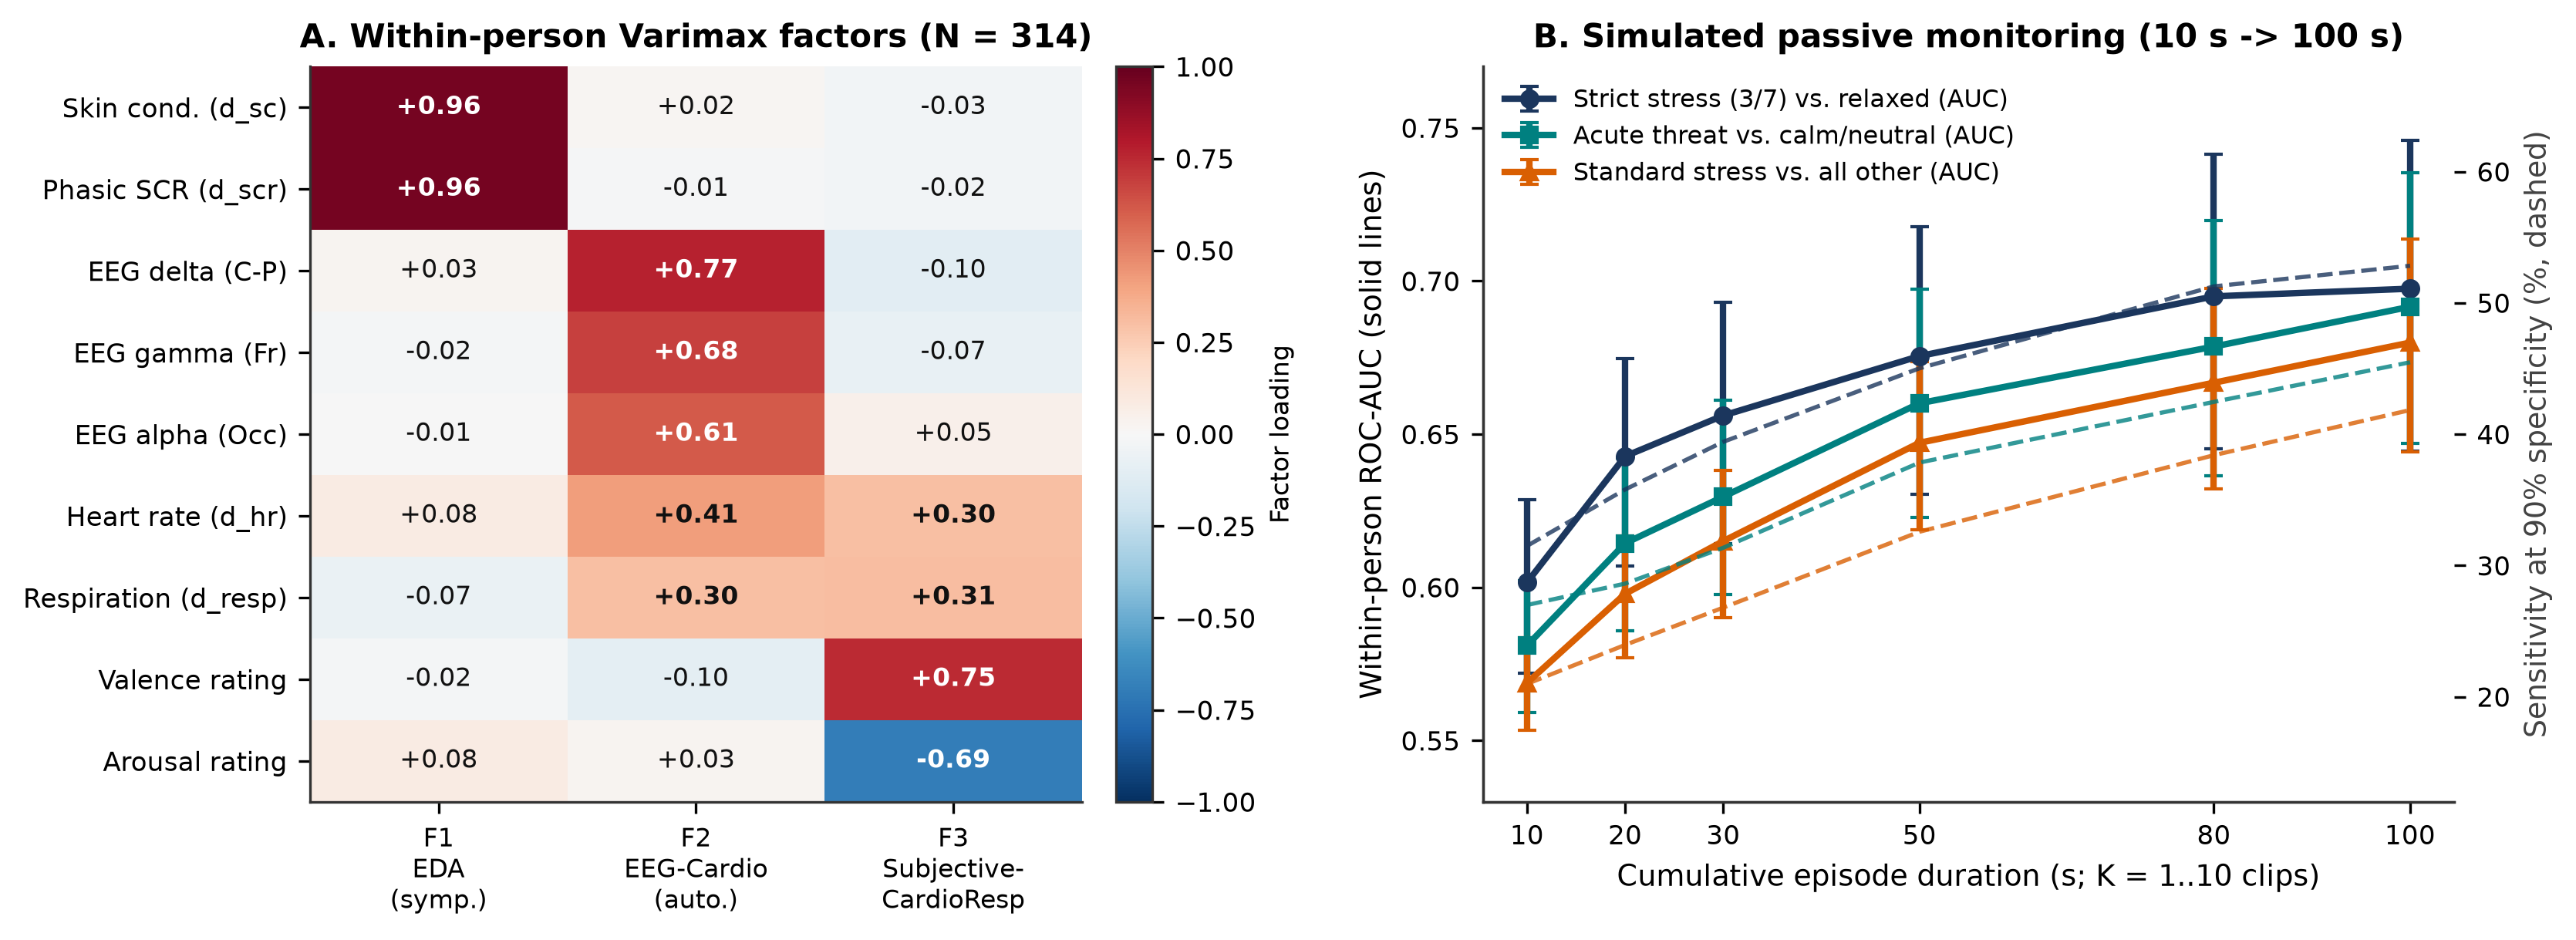
\includegraphics[width=.95\textwidth]{figures/fig4_coherence_monitoring.png}\end{center}
{\small Figure S1. Poids des composantes après rotation (gauche) et scores moyennés par classe connue (droite). Les courbes indiquent l’AUC et la sensibilité à un seuil propre à chaque identifiant. Sur cinq épisodes en blocs disjoints, l’AUC standard vaut 0,634 pour 148 identifiants. Les données ne permettent pas ce contrôle à dix épisodes.}
\section*{S5. Transfert, adaptation et reproductibilité}
Dans l’étude historique de transfert à une semaine, 103 identifiants étaient éligibles les deux jours. L’écart apparié d’AUC entre le deuxième et le premier jour vaut $-0{,}0392$ [$-0{,}0728$ ; $-0{,}0085$] pour l’EDA, $+0{,}0246$ [$-0{,}0062$ ; $0{,}0548$] pour l’EEG manuel et $+0{,}0041$ [$-0{,}0280$ ; $0{,}0373$] pour le modèle multimodal. Les stimuli et les conditions de séance peuvent contribuer. Sur une fin de séquence réservée au test, après 40 essais de calibration étiquetés, le Ridge réentraîné par personne perd 0,0530 d’AUC [différence $-0{,}0868$ ; $-0{,}0208$]. Le rappel vers les coefficients de population donne une différence de $-0{,}0011$ [$-0{,}0264$ ; $0{,}0233$] et CORAL, sans étiquettes, de $-0{,}0063$ [$-0{,}0146$ ; $0{,}0018$] (104 identifiants).

L’analyse historique avec REVE sur l’EEG prétraité donnait un gain de corrélation cardiaque positif dans cinq cohortes sur cinq (globalement $+0{,}0107$ [0,0071 ; 0,0145]). Trois IC par cohorte excluaient zéro ; les deux autres portaient sur 17 et 8 identifiants. Ce transfert interne excluait la cohorte sans masquer les thèmes. Plusieurs identifiants peuvent désigner la même personne entre cohortes.

Les deux corrélations publiées pour le RMSSD sur 5 s répondent à des questions différentes. Entre les phases précoce et tardive du clip, la corrélation moyenne intra-identifiant est 0,2239 [0,1987 ; 0,2482] (313 identifiants). Entre les 5 premières secondes d’un segment de tâche de 60 s et le segment parent, la corrélation médiane intra-enregistrement vaut 0,27394 (10\,263 segments candidats, 508 enregistrements).

\textbf{Indice de l’essai, par cohorte.} AUC linéaires hors pli : C1, 0,492 [0,458 ; 0,526] ($n=73$) ; C2, 0,497 [0,471 ; 0,523] (80) ; C3, 0,515 [0,457 ; 0,566] (16) ; C4, 0,515 [0,456 ; 0,571] (32) ; C5, 0,544 [0,453 ; 0,650] (7).

\smallskip
\small\href{https://github.com/mathiaschebbah/habs/actions/runs/45854683170}{Study 11, c1eadc5}\quad\href{https://github.com/mathiaschebbah/habs/actions/runs/44635398113/attempts/2}{Figure 1A, 9dfefdf}
\quad\href{https://github.com/mathiaschebbah/habs/actions/runs/44635461916/attempts/2}{RMSSD, 9dfefdf}
\quad\href{https://github.com/mathiaschebbah/habs/actions/runs/45091493959}{Video, 9989627}
\quad\href{https://github.com/mathiaschebbah/habs/actions/runs/45604993423}{Study 10, 51394bc}
\end{document}
